\documentclass{article}
\usepackage{amsmath}
\usepackage{graphicx}
\usepackage{hyperref}
\usepackage{physics}
\usepackage{tikz}
\usepackage{amsfonts}
\usepackage[most]{tcolorbox}
\usepackage[utf8]{inputenc}
\usetikzlibrary{calc}
% \usepackage[dvipsnames]{xcolor}

\definecolor{block-gray}{rgb}{0, 0.8, 0}
\newtcolorbox{answer}{colback=block-gray,grow to right by=-10mm,grow to left by=-10mm,
boxrule=0pt,boxsep=0pt,breakable}

% \graphicspath{ {images/} }

\title{Homework 4}
\author{Lev Kozlov}
\date{September 2022}

\begin{document}

\maketitle

\href{https://lvjonok.github.io/f22-theoretical-mechanics/2022/09/18/homework3.html}{Homework 4 webpage}

\subsection*{Task 1}

Too lazy to draw in tikz, so here you are.

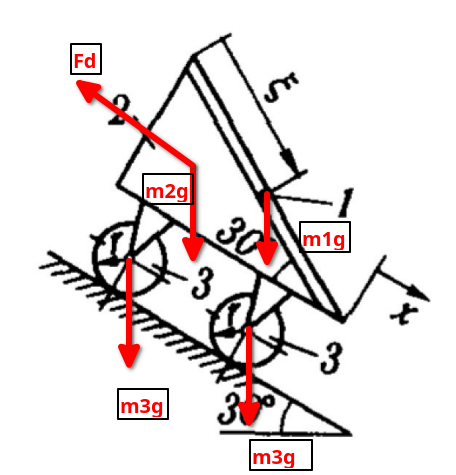
\includegraphics[width=\linewidth]{task1.png}

\subsubsection*{Part 1: find the angle to shoot the officer}

\begin{enumerate}
    \item RO: particle - planar motion
    \item Condition:
          \begin{center}
              \begin{tabular}{ |c|c|c| }
                  \hline
                  $$    & $initial$                & $final$                  \\
                  \hline
                  $t$   & $0$                      & $?$                      \\
                  \hline
                  $x$   & $0$                      & $L$                      \\
                  \hline
                  $x'$  & $v_0 \cdot \cos(\alpha)$ & $v_0 \cdot \cos(\alpha)$ \\
                  \hline
                  $x''$ & $0$                      & $0$                      \\
                  \hline
                  $y$   & $0$                      & $0$                      \\
                  \hline
                  $y'$  & $v_0 \cdot \sin(\alpha)$ & $?$                      \\
                  \hline
                  $y''$ & $-g$                     & $-g$                     \\
                  \hline
              \end{tabular}
          \end{center}
    \item Force analysis:
          $\vec{G}$
    \item Solution:
          \begin{enumerate}
              \item Equations by axis:
                    \begin{align}
                        \begin{cases}
                            mx'' = 0   \\
                            my'' = -mg \\
                        \end{cases}
                    \end{align}
                    Integration yields:
                    \begin{align}
                        \begin{cases}
                            x' = c_1       \\
                            y' = -gt + c_3 \\
                        \end{cases}
                    \end{align}
                    Another integration: \\
                    \begin{align}
                        \begin{cases}
                            x = c_1 t + c_2                    \\
                            y = -\frac{1}{2}gt^2 + c_3 t + c_4 \\
                        \end{cases}
                    \end{align}
              \item Substitution of initial values:
                    \begin{align}
                        \begin{cases}
                            c_1 = v_0 \cdot \cos(\alpha) \\
                            c_2 = 0                      \\
                            c_3 = v_0 \cdot \sin(\alpha) \\
                            c_4 = 0
                        \end{cases}
                    \end{align}
              \item Combining:
                    \begin{align}
                        \begin{cases}
                            L = v_0 \cdot \cos(\alpha) t \\
                            0 = -\frac{1}{2}gt^2 + v_0 \cdot \sin(\alpha) t
                        \end{cases}
                    \end{align}
              \item Result:
                    Python says there are two solutions: $\alpha = 0.0097$ and $\alpha = 1.561$.
                    And I have no doubts to not trust Python.
          \end{enumerate}
\end{enumerate}

\subsubsection*{Part 2: find the max height of the cargo ship can be to make this shot}

\begin{enumerate}
    \item As there are two angles that satisfy the first part, we need to find the max height for each of them.
    \item Analysis of equation for y-axis:
          \begin{align}
              y = -\frac{1}{2}gt^2 + v_0 \cdot \sin(\alpha) t
          \end{align}
    \item  As y is parabola, we can simply find its maximum height by finding extrema:
          \begin{align}
              t_{max} = \frac{v_0 \cdot \sin(\alpha)}{g} \\
              y_{max} = y(t_{max})
          \end{align}
    \item Result: \\
          For the first case: $y_{max} = 3.64555853045729$ \\
          For the second case: $y_{max} = 38574.3360928457$
\end{enumerate}

\subsubsection*{Part 3: find an angle $\alpha$, if you take into consideration the air resistance}

\begin{enumerate}
    \item RO: particle - planar motion
    \item Condition:
          \begin{center}
              \begin{tabular}{ |c|c|c| }
                  \hline
                  $$    & $initial$                & $final$ \\
                  \hline
                  $t$   & $0$                      & $?$     \\
                  \hline
                  $x$   & $0$                      & $L$     \\
                  \hline
                  $x'$  & $v_0 \cdot \cos(\alpha)$ & $?$     \\
                  \hline
                  $x''$ & $0$                      & $0$     \\
                  \hline
                  $y$   & $0$                      & $0$     \\
                  \hline
                  $y'$  & $v_0 \cdot \sin(\alpha)$ & $?$     \\
                  \hline
                  $y''$ & $-g$                     & $-g$    \\
                  \hline
              \end{tabular}
          \end{center}
    \item Force analysis:
          $\vec{G}$, $\vec{F}_{c}$
    \item Solution:
          \begin{enumerate}
              \item Equations by axis:
                    \begin{align}
                        \begin{cases}
                            mx'' = -k \sqrt{x'^2 + y'^2} x' \\
                            my'' = -mg - k \sqrt{x'^2 + y'^2} y'
                        \end{cases}
                    \end{align}
              \item Too hard to integrate by hands, so I'll use Python.
                    Everthing is the same as in part 1, but with different result.
              \item Result: \\
                    An angle to shoot officer is $\approx 0.0324$
          \end{enumerate}
    \item Air resistance force: \\
          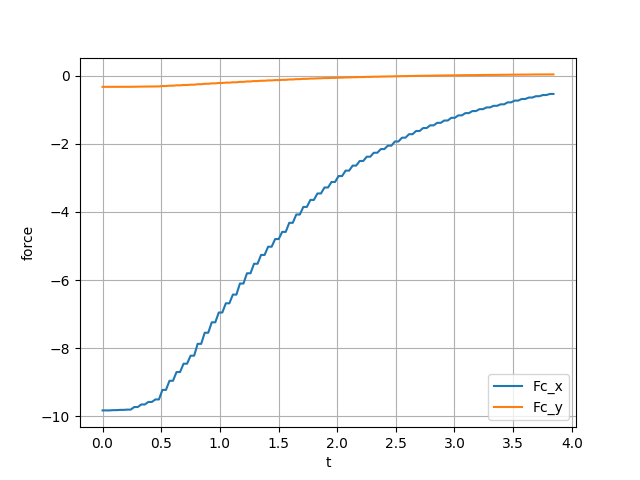
\includegraphics[width=\linewidth]{task1force.png}
    \item Trajectory with resistance: \\
          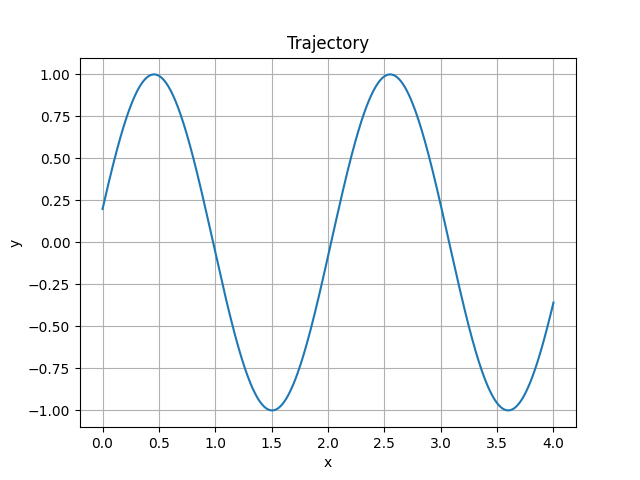
\includegraphics[width=\linewidth]{trajectory.png}
\end{enumerate}

\begin{answer}
    \begin{enumerate}
        \item
              $\alpha = 0.0097$, \\
              $\alpha = 1.561$
        \item
              $y_{max} = 38574.336$
        \item
              $\alpha = 0.0324$
    \end{enumerate}
\end{answer}


\newpage

\subsection*{Task 2}

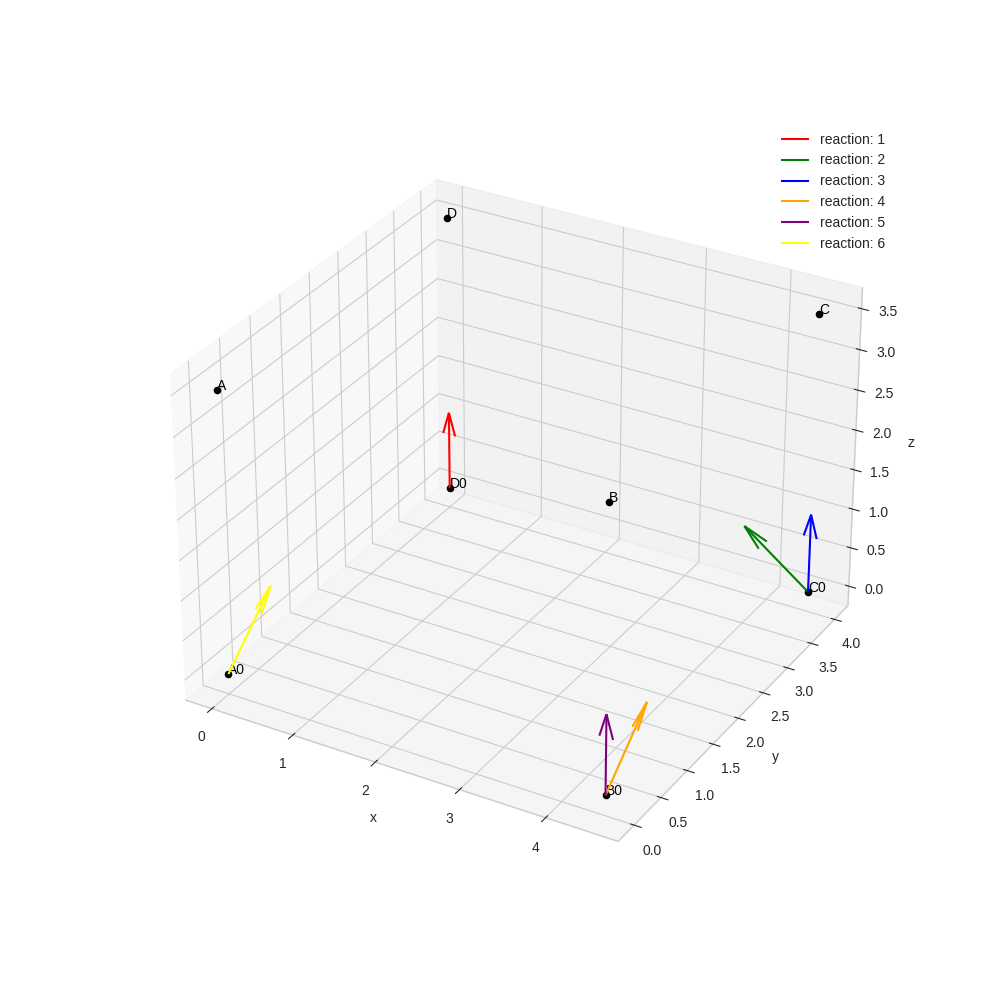
\includegraphics[width=\linewidth]{task2init.png}

\begin{enumerate}
    \item RO: system of 2 rods AB, BC
    \item Method: Theorem of change of kinetic energy (correlation between displacement and velocity)
    \item Force analysis:
          \[\vec{N}_a, \vec{N}_c, m_{AB}\vec{g}, m_{BC}\vec{g} \] \\
          There are no forces along x-axis $\implies$ B will hold its x position
    \item Conditions: \\
          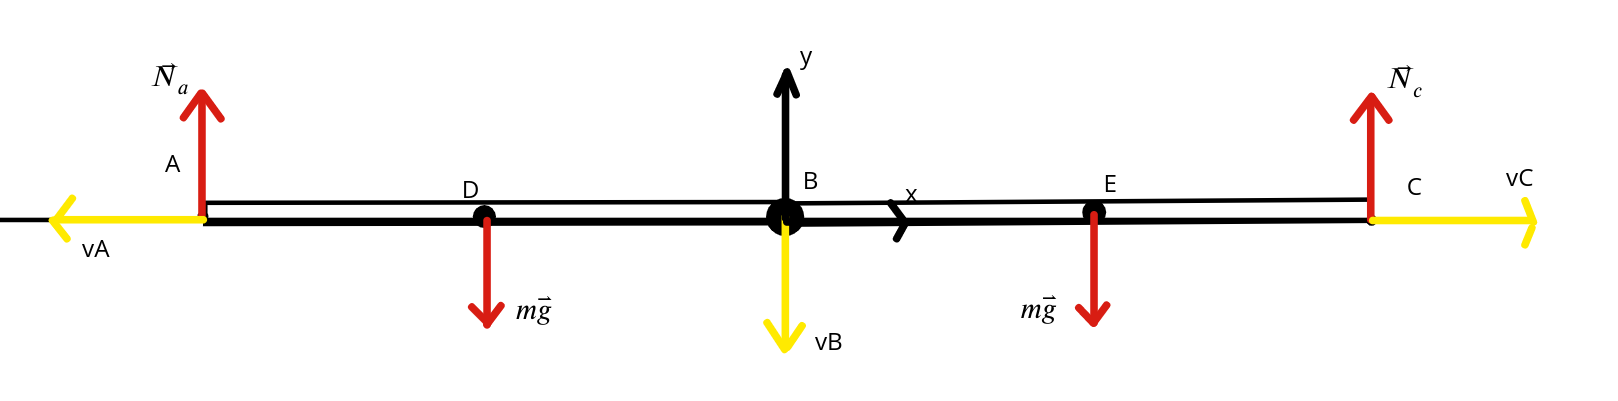
\includegraphics[width=\linewidth]{task2h.png}
          \begin{tabular}{|c|c|c|}
              \hline
              $$    & $initial$            & $final$                  \\
              \hline
              $x_b$ & $0$                  & $0$                      \\
              \hline
              $y_b$ & $h$                  & $0$                      \\
              \hline
              $x_c$ & $\sqrt{4l^2 - h^2}$  & $\sqrt{4l^2 - h^2} + h$  \\
              \hline
              $y_c$ & $0$                  & $0$                      \\
              \hline
              $x_a$ & $-\sqrt{4l^2 - h^2}$ & $-\sqrt{4l^2 - h^2} - h$ \\
              \hline
              $y_a$ & $0$                  & $0$                      \\
              \hline
          \end{tabular}
    \item Solution:
          \begin{enumerate}
              \item Kinetic energy:
                    \begin{align}
                        T_{AB} = \frac{1}{2}I\omega_{AB}^2 \\
                        T_{BC} = \frac{1}{2}I\omega_{BC}^2
                    \end{align}
              \item Inertia of the rod: \\
                    I will use Huygens–Steiner theorem to find moment of inertia. \\
                    \begin{align}
                        I = m_{AB}l^2 + m_{AB}\rho^2
                    \end{align}
              \item Angular velocity of the rods: \\
                    IC of velocity for rod $AB$ at the final will be at $A$, $BC$ at $C$. \\
                    \begin{align}
                        v_B = \omega_{AB} \cdot 2l \\
                        v_B = \omega_{BC} \cdot 2l
                    \end{align}
              \item Work done by external forces: \\
                    \begin{align}
                        A_{if} = mg \frac{h}{2} + mg \frac{h}{2}
                    \end{align}
              \item Equation of change:
                    \begin{align}
                        T_{AB} + T_{BC} = A_{if}                                                                                        \\
                        \frac{1}{2}I \cdot (\frac{v_B}{2l})^2 + \frac{1}{2}I \cdot (\frac{v_B}{2l})^2 = mg \frac{h}{2} + mg \frac{h}{2} \\
                        v_B = 2l \sqrt{\frac{gh}{l^2 + \rho^2}}
                    \end{align}
          \end{enumerate}
\end{enumerate}

\subsection*{Task 2 (next part)}

This part is pretty much the same as the previous one, but with a different final conditions.

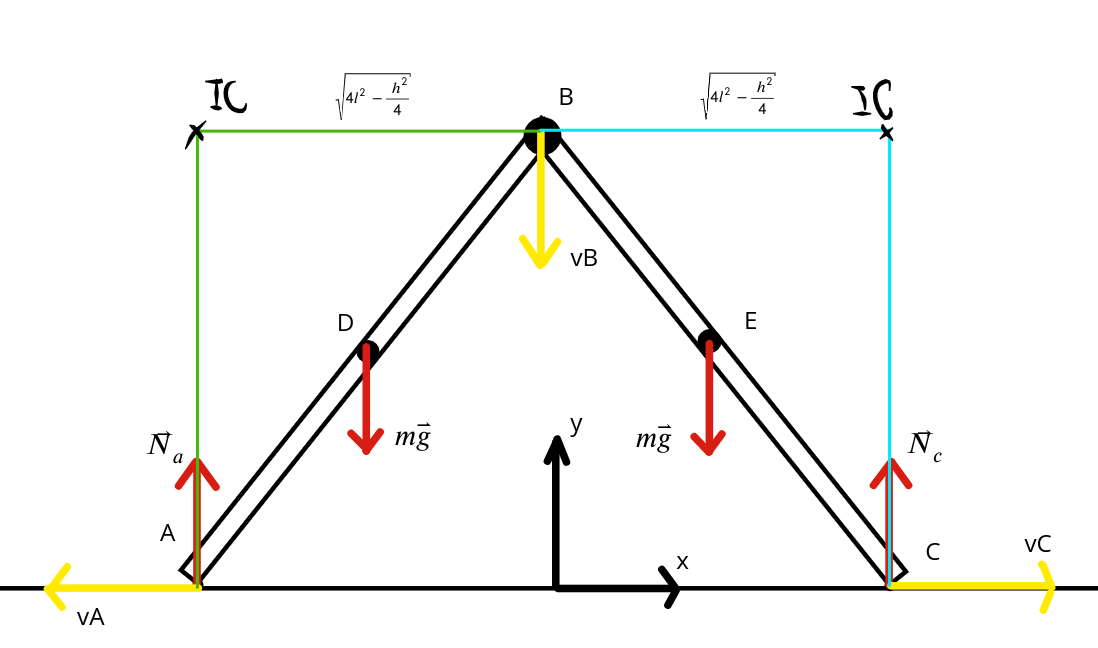
\includegraphics[width=\linewidth]{task2ic.png}

\begin{enumerate}
    \item Conditions: \\
          \begin{tabular}{|c|c|c|}
              \hline
              $$    & $initial$            & $final$                    \\
              \hline
              $x_b$ & $0$                  & $0$                        \\
              \hline
              $y_b$ & $h$                  & $h/2$                      \\
              \hline
              $x_c$ & $\sqrt{4l^2 - h^2}$  & $\sqrt{4l^2 - h^2} + h/2$  \\
              \hline
              $y_c$ & $0$                  & $0$                        \\
              \hline
              $x_a$ & $-\sqrt{4l^2 - h^2}$ & $-\sqrt{4l^2 - h^2} - h/2$ \\
              \hline
              $y_a$ & $0$                  & $0$                        \\
              \hline
          \end{tabular}
    \item Angular velocities of the rods: \\
          IC is shown on picture above: \\
          \begin{align}
              v_B = \omega_{AB} \cdot \sqrt{4l^2 - \frac{h^2}{4}} \\
              v_B = \omega_{BC} \cdot \sqrt{4l^2 - \frac{h^2}{4}}
          \end{align}
    \item Work done by external forces: \\
          \begin{align}
              A_{if} = mg \frac{h}{4} + mg \frac{h}{4}
          \end{align}
    \item Equation of change:
          \begin{align}
              T_{AB} + T_{BC} = A_{if}                                                                                                                                                  \\
              \frac{1}{2}I \cdot \big(\frac{v_B}{\sqrt{4l^2 - \frac{h^2}{4}}}\big)^2 + \frac{1}{2}I \cdot (\frac{v_B}{\sqrt{4l^2 - \frac{h^2}{4}}})^2 = mg \frac{h}{4} + mg \frac{h}{4} \\
              v_B = \frac{1}{2} \sqrt{16l^2 - h^2} \sqrt{\frac{gh}{2 (l^2 + \rho^2) }}
          \end{align}
\end{enumerate}

\subsubsection*{Answer:}

\begin{answer}
    \begin{enumerate}
        \item \begin{align}
                  v_B = 2l \sqrt{\frac{gh}{l^2 + \rho^2}} \notag
              \end{align}
        \item \begin{align}
                  v_B = \frac{1}{2} \sqrt{16l^2 - h^2} \sqrt{\frac{gh}{2 (l^2 + \rho^2) }} \notag
              \end{align}
    \end{enumerate}
\end{answer}



\end{document}